Last time, we wrote down a counterterm action to cancel UV divergences at one-loop order:
\begin{equation*}
    S^{CT}[\phi,\Lambda]=\int d^4x \bkt{
        \frac{\delta Z(\Lambda)}{2} \p_\mu \phi \p^\mu \phi +\frac{1}{2} \delta m^2(\Lambda) \phi^2 +\frac{\delta \lambda(\Lambda)}{4!} \phi^4
    }.
\end{equation*}
Using our on-shell renormalization scheme, we chose
\begin{gather*}
    \delta Z=0,\\
    \delta m^2= -\frac{\lambda}{32\pi^2} \bkt{\Lambda^2-m^2\log \paren{1+\frac{\Lambda^2}{m^2}}}.
\end{gather*}
To determine $\delta \lambda$, we must look at the $1$-loop level correction to the quartic coupling, $\frac{\lambda}{4!}\phi^4$. Before considering any counterterms, there are three diagrams%
    \footnote{Diagram credit to \href{http://www.damtp.cam.ac.uk/user/dbs26/AQFT/chap5.pdf}{Skinner}, \textsection 5.1.2.}
which modify the quartic coupling:
\begin{center}
    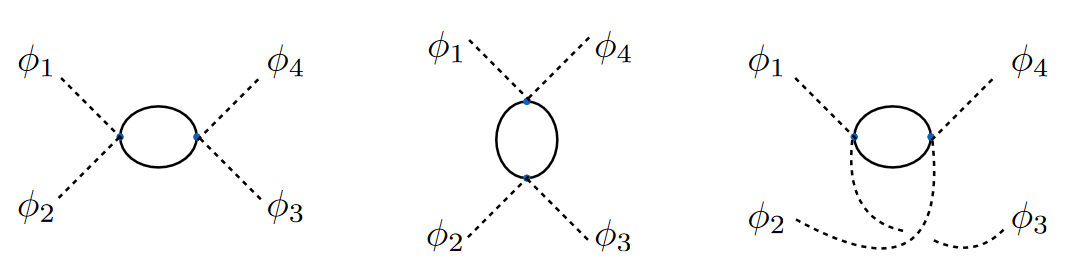
\includegraphics{2019/02/20190212_skinnerquartic.png}
\end{center}
which correspond to an amplitude
\begin{equation}
    \frac{\lambda^2}{2} \int^\Lambda \frac{d^4k}{(2\pi)^4}\frac{1}{k^2+m^2} \bkt{
        \frac{1}{(p_1+p_2+k)^2 +m^2}
        +\frac{1}{(p_1+p_4+k)^2+m^2}
        +\frac{1}{(p_1+p_3+k)^2+m^2}
    }.
\end{equation}
The overall factor of $1/2$ is a symmetry factor since the two internal lines are identical and can be exchanged, and the propagators can be read off by conservation of momentum at each vertex (taking all external momenta to be flowing in). We can evaluate this integral in terms of the external momenta $p_i$, but let's try to get a feel for the divergence first. We see that this integral goes as $d^4k/k^4$, so we expect a $\log\Lambda$ divergence. More precisely, the large $k$ behavior (where we care about this divergence) will look like%
    \footnote{This integral isn't totally immediate. To evaluate this, rewrite $k^3 dk= \frac{1}{2}k^2 d(k^2)$. Next, divide through in the numerator and denominator by $m^4$ to get
    \begin{equation*}
        \frac{1}{2}\int_0^\Lambda \frac{(k^2/m^2) d(k^2/m^2)}{(k^2/m^2) +1)^2}=\frac{1}{2}\int_0^{\Lambda^2/m^2} \frac{u\,du}{(u+1)^2}.
    \end{equation*}
    Finally, to evaluate the $u$ integral, just integrate by parts. Some similar integrals like $\int \frac{u\, du}{1+u}$ are amenable to a simple rewriting as $\frac{u}{1+u}=1-\frac{1}{1+u}$, but in general you'll want to integrate by parts:
    \begin{equation*}
        \int_0^{\Lambda^2/m^2} u\frac{du}{(1+u)^2}= -\left.\frac{u}{1+u}\right\rvert_0^{\Lambda^2/m^2} -\int \paren{-\frac{1}{1+u}}du=-\left.\frac{u}{1+u}\right\rvert_0^{\Lambda^2/m^2} +\left.\log(1+u)\right\rvert_0^{\Lambda^2/m^2}=\log\paren{1+\frac{\Lambda^2}{m^2}}-\frac{\Lambda^2}{\Lambda^2+m^2}.
    \end{equation*}
    
    }
\begin{align}
    \frac{3\lambda^2}{2} \int^\Lambda \frac{d^4k}{(2\pi)^4}\frac{1}{(k^2+m^2)^2} &= \frac{3\lambda^2}{16\pi^3} \int_0^\Lambda \frac{k^3 dk}{(k^2+m^2)^2}\\
    &= \frac{3\lambda^2}{32\pi^2} \int_0^{\Lambda^2/m^2} \frac{u\,du}{(1+u)^2}\\
    &= \frac{3\lambda^2}{32\pi^2} \bkt{
        \log\paren{1+\frac{\Lambda^2}{m^2}}-\frac{\Lambda^2}{\Lambda^2+m^2}\label{quarticdivergence}
    }.
\end{align}
This value is the shift in the $\lambda$ coupling before we introduce the $\delta \lambda$ counterterm.
If we then choose
\begin{equation}
    \delta \lambda =\frac{3\lambda^2}{32\pi^2} \bkt{\log \frac{\Lambda^2}{m^2}-1},
\end{equation}
we can then produce an effective coupling of 
\begin{equation}
    \lambda_{\text{eff}}=\lambda -\frac{3\lambda^2}{32\pi^2} \bkt{\log \paren{1+\frac{m^2}{\Lambda^2}}+\frac{m^2}{m^2+\Lambda^2}},
\end{equation}
which is finite as $\Lambda\to\infty$.%
    \footnote{
        This is just $\lambda$ plus the one-loop correction we computed to be \ref{quarticdivergence} plus our choice of $\delta \lambda$ (which is itself treated as a one-loop correction). In fact, there's a relative minus sign between the original coupling and the one-loop correction. That is, the original coupling contributes $(-\lambda \delta^{(4)}(\ldots)$, while the one-loop diagrams contribute $(-\lambda)^2 \delta^{(4)}(\ldots)$. Thus
        \begin{align*}
            \lambda_\text{eff}&=\lambda -\frac{3\lambda^2}{32\pi^2} \bkt{
                \log\paren{1+\frac{\Lambda^2}{m^2}}-\frac{\Lambda^2}{\Lambda^2+m^2}
            }
            +\frac{3\lambda^2}{32\pi^2} \bkt{\log \frac{\Lambda^2}{m^2}-1}\\
            &= \lambda -\frac{3\lambda^2}{32\pi^2} \bkt{\log \paren{1+\frac{m^2}{\Lambda^2}}+\frac{m^2}{m^2+\Lambda^2}}.
        \end{align*}
    }

Having computed the log divergence one way, let us try to be a little more precise and account for the external momenta. For this next discussion, we'll need a trick due to Feynman:
\begin{equation}
    \int_0^1 \frac{dx}{\bkt{xA+(1-x)B}^2} =\frac{1}{B-1} \bkt{\frac{1}{xA+(1-x)B}}_0^1 = \frac{1}{AB}.
\end{equation}
We'll use this to rewrite products of denominators (i.e. propagators) as these sorts of integrals, i.e. from right to left. Note that the integral can be put in a more manifestly symmetric form as
\begin{equation*}
    \int_0^1 dx \int_0^1 dy \frac{\delta(x+y-1)}{(xA+yB)^2}.
\end{equation*}

To compute the loop integral for our first diagram, let $p_{12}\equiv p_1 +p_2$. Using Feynman's trick, we can rewrite the propagators as
\begin{align*}
    \frac{1}{(p_{12}+k)^2+m^2}\frac{1}{k^2+m^2}&=\int_0^1 \frac{dx}{\bkt{x((p_{12}+k)^2+m^2)+(1-x)(k^2+m^2)}^2
    }\\
        &= \int_0^1 \frac{dx}{\bkt{(k+xp_{12})^2 +m^2 +x(1-x)p_{12}^2}^2}\\
        &= \int_0^1 \frac{dx}{\bkt{l^2+m^2+x(1-x)p_{12}^2}^2}
\end{align*}
where we have defined $l=k+x p_{12}$ and completed the square.
In the $\Lambda \to \infty$ limit, the shifted integration range $|k|\leq \Lambda \to |l|\leq \Lambda$ vanishes, so we can turn our $d^4k$ integral into a $d^4 l$ and write
\begin{align*}
    \int \frac{d^4ldx}
    {\bkt{l^2+m^2+x(1-x)p_{12}^2}^2}
    &= S_4 \int_0^1 dx \int_0^\Lambda \frac{l^3 dl}
    {\bkt{l^2+m^2+x(1-x)p_{12}^2}^2}\\
    &= \pi \int_0^1 dx \set*{ \log \bkt{
        \frac{\Lambda^2 +m^2+x(1-x)p_{12}^2}{m^2+m^2+x(1-x)p_{12}^2}
    }
    +\frac{m^2+x(1-x)p_{12}^2}{\Lambda^2+m^2+x(1-x)p_{12}^2}
    -1
    }
\end{align*}
after a change of variables and an integration by parts. Note that this term with the $1/\Lambda^2$ goes to zero as $\Lambda\to\infty$, so we will not need to worry about renormalizing it. We also notice that all three diagrams are related by the Mandelstam variables 
\begin{equation}
    s=-(p_1+p_2)^2,\quad t=-(p_1+p_4)^2, \quad u=-(p_1+p_3)^2,
\end{equation}
so that the sum of our three diagrams (restoring prefactors) is then
\begin{equation}
    \frac{\lambda^2}{32\pi^2}\int_0^1 dx \set*{ \log \paren{\frac{\Lambda^2}{m^2-x(1-x)s}} 
    + \log \paren{\frac{\Lambda^2} {m^2-x(1-x)t}}
    + \log \paren{\frac{\Lambda^2} {m^2-x(1-x)u}}
    -3
    }.
\end{equation}
The coefficient of $\tilde \phi^4$ in the effective action $\Gamma(\tilde \phi)$ (i.e. $\tilde \phi$ in momentum space) is
\begin{equation}
    \lambda+\delta \lambda -\frac{\lambda^2}{32\pi^2} \int d \set{\ldots}
\end{equation}
with $\delta \lambda$ from above, and replacing $(m^2,\lambda)\mapsto (m_{\text{phys}}^2,\lambda_{\text{eff}})$.
We find that 
\begin{equation}
    \lambda_{\text{eff}}+\frac{\lambda_{\text{eff}}^2}{32\pi^2} \int_0^1 dx \set*{ \log \bkt{1-\frac{x(1-x)s}{m_{\text{phys}}^2}}
    +\log \bkt{1-\frac{x(1-x)t}{m_{\text{phys}}^2}}
    +\log \bkt{1-\frac{x(1-x)u}{m_{\text{phys}}^2}}
    }
\end{equation}
is finite-- no more counterterms are necessary after $\delta m^2$ and $\delta \lambda$. Our capacity to regulate these terms depends on the idea of operators being relevant, irrelevant, or marginal (depending on their mass dimension as compared to the dimension of spacetime).